\chapter{Simulation Result}

In the first section, we will have an overview on our simulation program and our testing environment. Then in the following section, the simulation results and analysis will be presented as the concept proof of our new approach. 


\section{Overview}

In this section, we will have an overview on our simulation program and our testing configuration. 

Our simulation program is implemented with CUDA, the host part of the code is fully written in C++ and the code running by GPU is written in CUDA C which is an extension of standard C programming language. All of the code for GPU kernels is encapsulated in separated files(*.cu).

Several 3rd party frameworks are employed for a variety of features. Open Asset Import Library(Assimp) is an open source library to import various well-known 3D models formats. It is written in C++ and very easy to integrate with our code. Another important framework we used is wxWidget. wxWidget is C++ based cross-platform light-weight Graphics User Interface(GUI) toolkits. We use it for the UI and displaying the final render result. 

\subsection{System Specification}

The testing system's specificaiton is listed in the table \ref{tab:sys_spec} :

\begin{table}[!ht]
\begin{center}
	\begin{tabular}{ | l | l |}     	
	\hline 

	CPU					& 		Intel Core i7 2620M 2.7GHz		\\ 
	\cline{1-2}
	System Memory  		& 		8GB DDR3 						\\ 
	\cline{1-2}
	GPU 					& 		nVidia Quadro 2000M 			\\
	\cline{1-2}
	GPU Memory 			& 		2GB DDR3						\\
	\cline{1-2}
	CUDA Cores			& 		192 							\\  
	\cline{1-2}
	CUDA Version 			&		4.0							\\ 
	\cline{1-2}
	Driver Version  		&		296.88						\\ 
	\hline

	\end{tabular}
\end{center} 
\caption{System Specification}
\label{tab:sys_spec}
\end{table}

\subsection{Application Specification}

In our test program, the following key features are implemented: 

\begin{itemize}

\item{GPU-based(CUDA) Monte-Carlo ray tracing and kd-tree implementation.}

\item{GPU-based(CUDA) photon mapping technique. } 

\item{GPU-based(CUDA) photon mapping with kd-tree leaf nodes photon queue.} 

\item{Use CUDA-OpenGL interop for the final render result display. }

\end{itemize}

We use the CUDA Toolkit 4.2 and Microsoft Visual Studio 2012 as the base CUDA development environment, the build target is release and all default optimizations are turned on. 

\subsection{Test Scene Specification}


\section{Data Structure Construction}
\label{sec:build_time}

Firstly, we will look at the performance of the data structure construction. Given a total number of photons shot in the scene, we compare the constructiona time among a range of frames. As shown in figure \ref{fig:construction_time}, the construction time of the brute force(red curve)  the red curve indicates the construction time with the brute force method, that is we rebuild the kd-tree for photon map every frame from scratch with all the photons shot from the light source in the scene. The green curve represents the construction time using our increamental update approach. For each frame, we trace less photons(500 photons instead of 5000 in this test case) and keep accumulating the photons for rendering the following frames. Also the complicated kd-tree construction process is avoided. Therefore we can see the data structure construction time is shorter than the brute force method. 


\begin{figure}[ftp] 
    \centering 
    \fbox{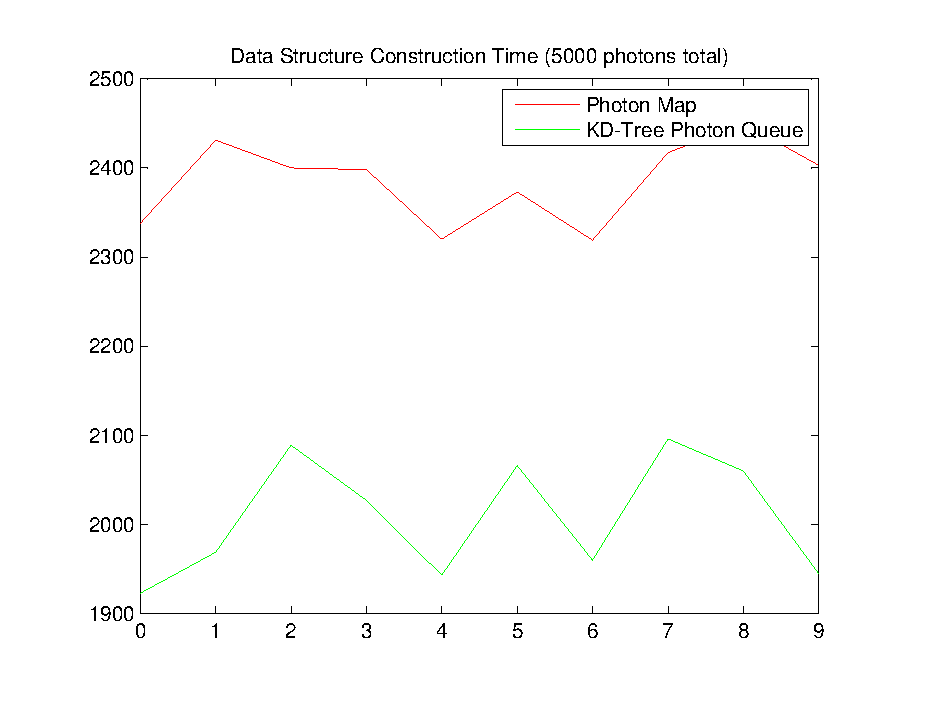
\includegraphics[width=\linewidth]{imgs/construction_time.pdf}}
    \renewcommand{\thefigure}{\thechapter.\arabic{figure}}
    \caption[]{Data structure construction time}
    \label{fig:construction_time} 
\end{figure} 

\section{Memory Consumption} 

The memory consumption is another important aspect we need to investigat. The memory capacity of the PC's video cards nowadays has been greatly extended, it is fairly easy to find an affordable video cards featured with 1024MB DDR5 on-board memory. However video memory is stil a type of valuable resource. When analysing the memory consumption of our technique compares to the brute force approach, we are looking at the data from two different running phases of our test program, the pre-rendering phase and rendering phase. 

As shown in figure \ref{fig:memory_consumption}, given the parameter of \emph{max frames} as \emph{10}, the memory consumption of our technique is considerably larger than the brute force, in fact, it requires more than 10 times more memory. The reason for this behavior is that we maintain a large buffer that works like circular buffer to keep track of all the photons data of previous frames, and the capacity of the buffer is determined by maximum number of frames we check back. In addition to the extra photon data, we also need to store another buffer on GPU memory that stores the photons that belongs to a kd-tree leaf node using photon indices which point to the photon data, buffer. Though the index is just represented with an 32-bit unsigned integer value which is much smalle than the detailed representation of a photon in the global buffer. 

\begin{figure}[ftp] 
    \centering 
    \fbox{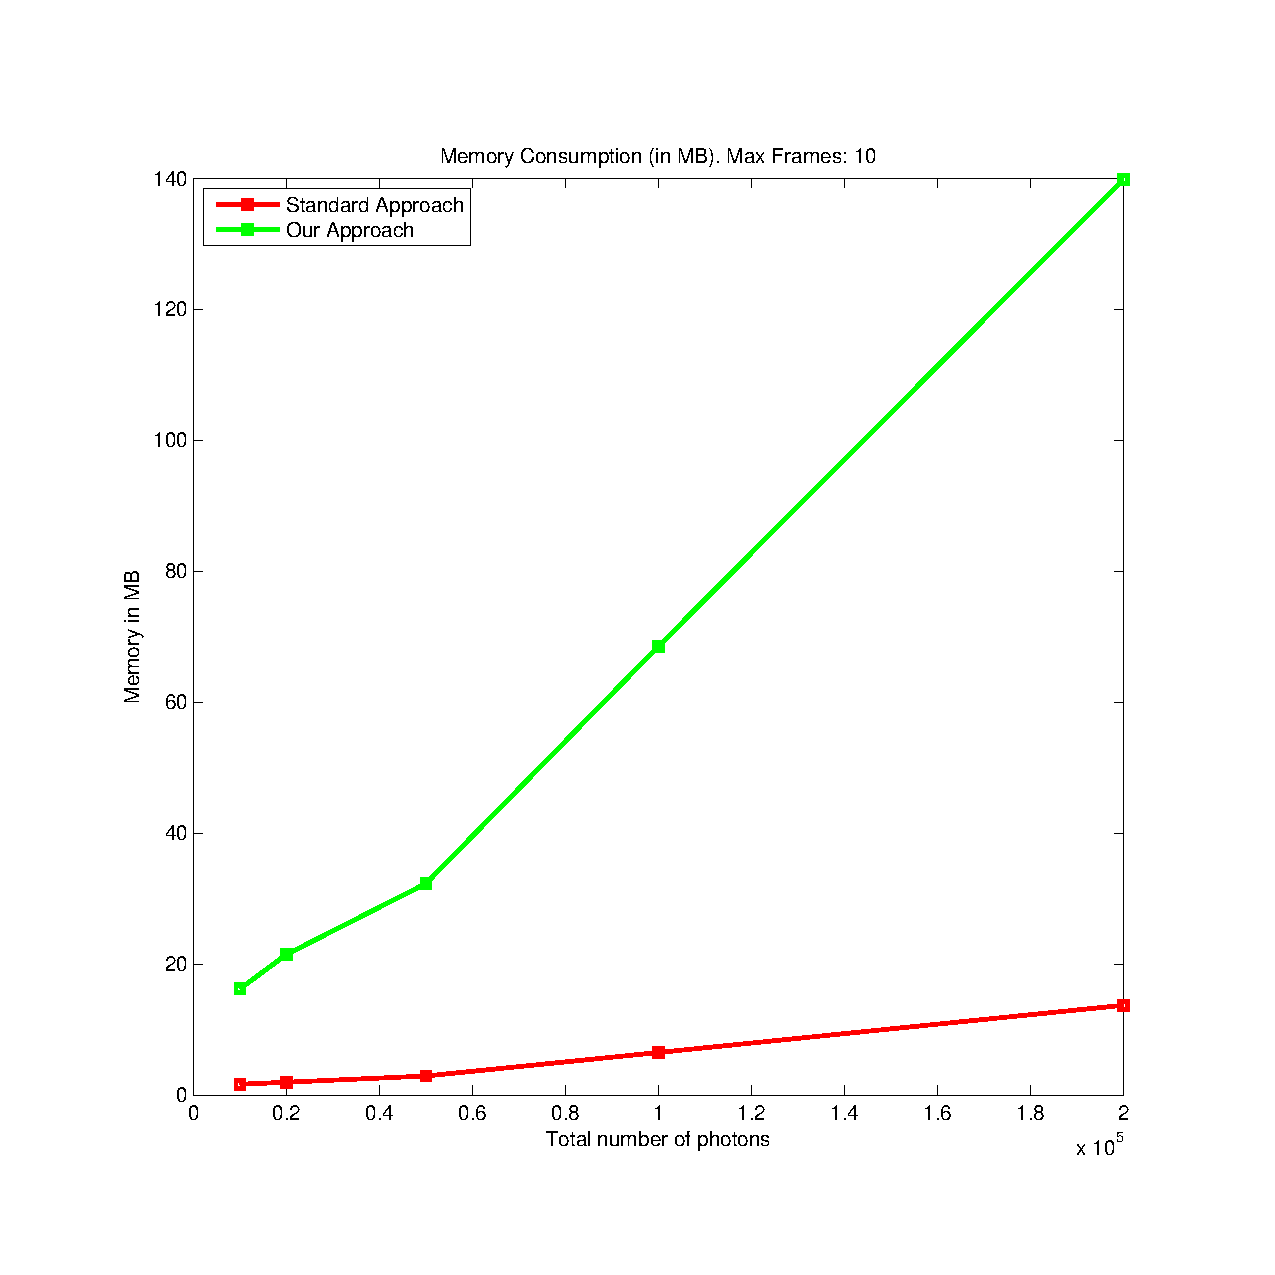
\includegraphics[width=\linewidth]{imgs/memory_consumption.pdf}}
    \renewcommand{\thefigure}{\thechapter.\arabic{figure}}
    \caption[]{Memory consumption in rendering phase.}
    \label{fig:memory_consumption} 
\end{figure}  

Although our new technique demands much more memory than the brute force does in the rendering phase, the memory requirement of our method is much lower than the brute force approach. This behavior is due to the big memory overhead introduced in kd-tree construction phase. Large amount of memory is allocated for the miscellaneous data structure such as the node list, the indices of triangles(triangles and points) and split list, and then will be released when construction is done. While our new technique does not require much temporary data. 

\begin{figure}[ftp] 
    \centering 
    \fbox{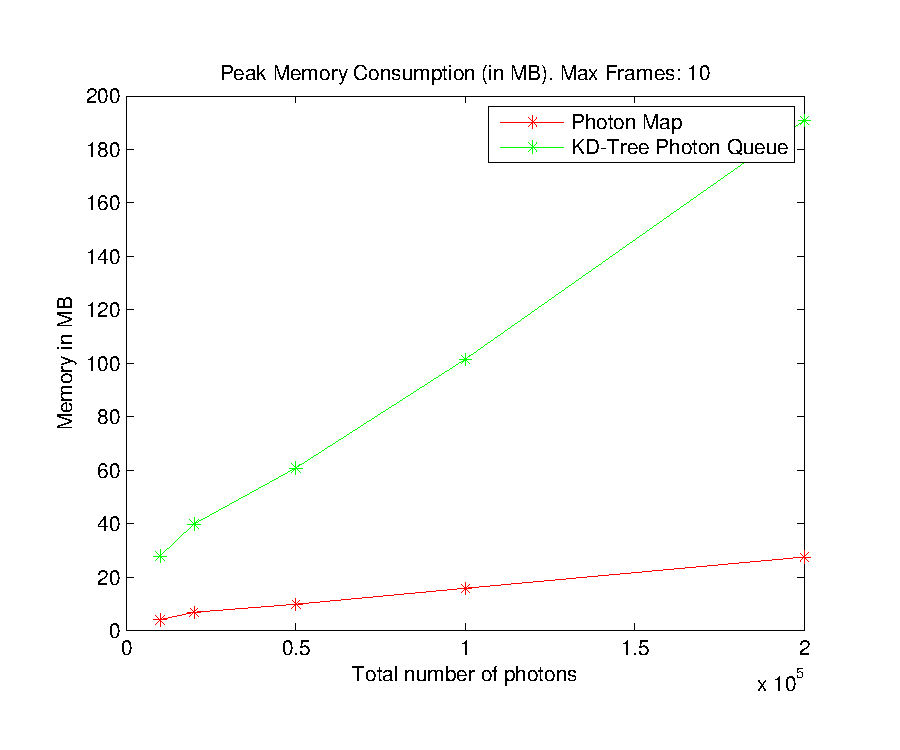
\includegraphics[width=\linewidth]{imgs/memory_consumption_2.pdf}}
    \renewcommand{\thefigure}{\thechapter.\arabic{figure}}
    \caption[]{Memory consumption in pre-render phase. }
    \label{fig:memory_consumption_2}  
\end{figure}   


As shown in figure \ref{fig:memory_consumption_2}, building a kd-tree for the photons demands much more memory than building the photons queue, even though the memory allocated here will release later, the peak memory consumption could bottleneck the performace of the whole program or even prevent the program from running for some video cards with smaller memory capacity. Since memory allocation is an expensive routine and kd-tree construction requires lots of temporary memory allocation/release, it becomes another important factor that brings negative impact on performance of the data structure construction for the brute force as we can see in the section \ref{sec:build_time}.  

\section{Photons Search}

In this section, we will show how the different techniques perform during the photon search. There are couple of parameters that have influence on the performance: 

\begin{itemize}

\item{The number of photons to search. }

\item{The search radius(maximum allowd distance between the query point and a photon). } 

\end{itemize} 

We will present how these parametes effect the photon search result and analyse the possible cause. 

\subsection{Number of Photons} 

As shown in the figure \ref{fig:photon_search_1}, the photon gathering of our technique is slightly faster than the standard photon mapping when number of photons is less than 150000, as the range of photons to search grows, it slows down and is out performed. As introduced earlier, our technique creates a buffer holding the photons that spatially belong to the leaf nodes of kd-tree for the scene objects, when performing the photon search, we traverse this built kd-tree with k-nearest neighbor algorithm to quickly reach the leaf nodes that is connecting with the photons that potentially fall into a pre-defined search range from the query point using the bouding box information of the kd-tree leaf nodes, then perform a linear search at this level. Compares to kd-tree built for the hundreds of thousands of photons in the scene, the kd-tree for geometry is usually far more coarse, especially for a relative simple scene. Therefore the kd-tree for a simple scene will have a small depth and a leaf node could have an large extent and holds a large number of photons. Thus the advantages of the binary search is out-weighted by the linear search. This is a possible reason why we have a result shown in figure \ref{fig:photon_search_1}. In an extreme case, when there is no split in the scene, thus the kd-tree only have one node, the root node which contains everything, the photon search will be degenerated into a linear search. 

\begin{figure}[ftp] 
    \centering 
    \fbox{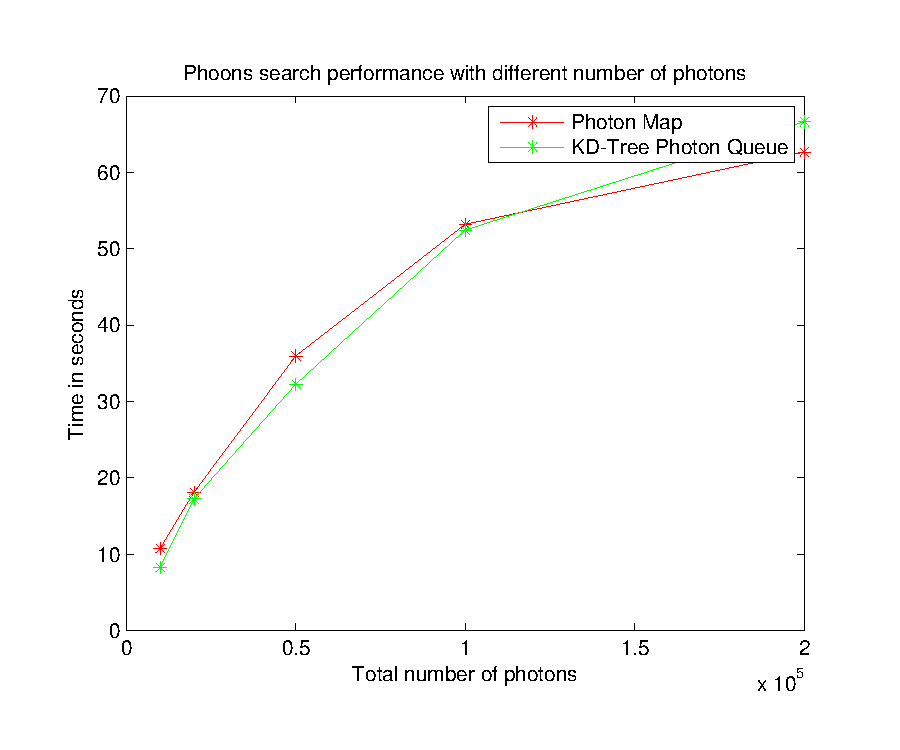
\includegraphics[width=\linewidth]{imgs/photon_search_1.pdf}}
    \renewcommand{\thefigure}{\thechapter.\arabic{figure}}
    \caption[]{Photon search performance with different number of photons. }
    \label{fig:photon_search_1}  
\end{figure} 

\subsection{Query Radius}

Figure \ref{fig:photon_search_2} shows that how the query radius effect the photon search performance. The standard photons search algorithm and our technique both have an almost steady increase in search time with an increasing query radius. For standard photon mapping method, since more kd-tree node will be enqueued to the stack waiting to be visited as the query radius increases, this brings larger kd-tree traversal overhead. When using photons queue for range search, the lost of performance becomes less than the standard photon mapping. As explained earlier, more photons are associated with one kd-tree leaf nodes, thus there are less nodes pushed to the local stack and the overhead of traversing the kd-tree is avoided. 

\begin{figure}[ftp] 
    \centering 
    \fbox{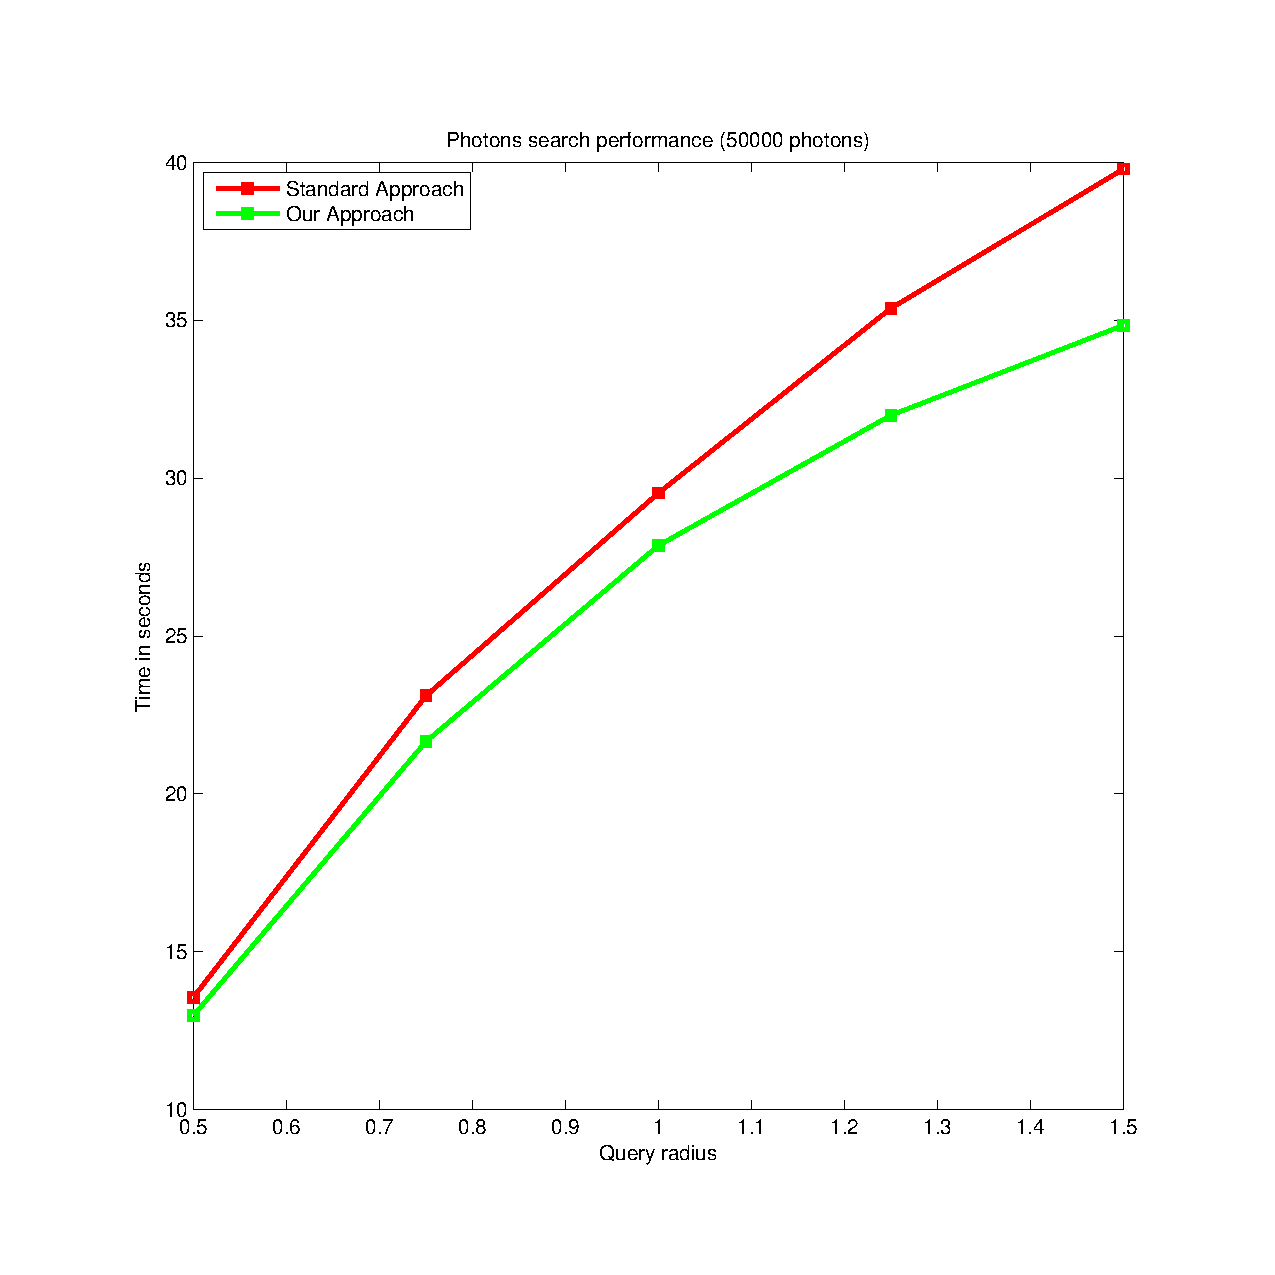
\includegraphics[width=\linewidth]{imgs/photon_search_2.pdf}}
    \renewcommand{\thefigure}{\thechapter.\arabic{figure}}
    \caption[]{Photon search performance with different query radius. }
    \label{fig:photon_search_2}  
\end{figure} 


\section{Overall Performance} 


\section{Image Quality}

In this section we take a look at the quality of our approach. As described in chapter 3, our new approach uses an increamental scheme to update the kd-tree and photons queue for the rendering to be beneficial for the dynamic scene with moving light source. Therefore it makes more sense to look at the result images of a range of frames to see the image quality, the light source will also be moving in the frame sequence so that we can see the change of equilibrium distribution of radiance in the scene. To obtain a better knowledge on how the photons are distributed in the scene each frame, we will present the photons visualization result images as well along with the result image. 

Several key parameters defined in our experiments for both the standard photon mapping method and our new approach are presented in the table \ref{tab:expr_params}. 

\begin{table}[ht]
\begin{center}
	
	\renewcommand{\arraystretch}{1.2}
	\begin{tabular}{p{5cm}p{3cm}p{5cm}}
	
	Parameter  				& 		Default Value 		&		Discription \\ 
	
	\hline 

	Max. Photons Bounses		& 		3					&		The maximum photons reflection will be traced. \\  

	\hline 					

	Total Number of Photons 	& 		200000				&		The total number of photons emitted from the light 																	source. \\

	\hline

	Light Source Type			& 		Point Light			& 		The type of light source, point light and area light
																are supported. However in this experiments only point 																	light is used. \\ 
	
	\hline
	
	Light Source Position 		& 	 	(0.0, 10.0, 0.0)		&		Default light source position in the scene. \\  


	\hline 
	
	Light Emission Intensity	&		(1.0, 1.0, 1.0)		&		The RGB representation of light emitted radiance.\\  

	\hline 

	Maximum Frames Counter 	& 		10 					& 		The maximum number of frames we keep track of. Given 																	the total number of photons as 200000, the photons 																	emitted for each frame is 20000\\

	\hline
	
	Image Resolution 			&		512 x 512				&		The resolution of result image. \\

	\hline 
	
	Samples per Pixel			& 		1 					& 		Multi-sampling is not used in the experiments thus 																	there is only 1 ray being traced per pixel.\\
	
	\hline 
	
	Trace Shadow Rays			&		Off					& 		Toggle tracing the shadow rays. \\

	\hline

	Specular Reflection		&		Off					&		Toggle of specular reflection when tracing photons. \\

	\hline
	
	\end{tabular}
\end{center} 
\caption{Experiments Parameters}
\label{tab:expr_params}
\end{table}

In figure \ref{fig:pm_global}, we firstly present the result image rendered with default values of the parameters listed in table \ref{tab:expr_params} using standard photon mapping algorithm and phtons visualization image. 

\begin{figure}[htp] 
    \centering 
    \fbox{
	\subfigure[Test subfigure 1]{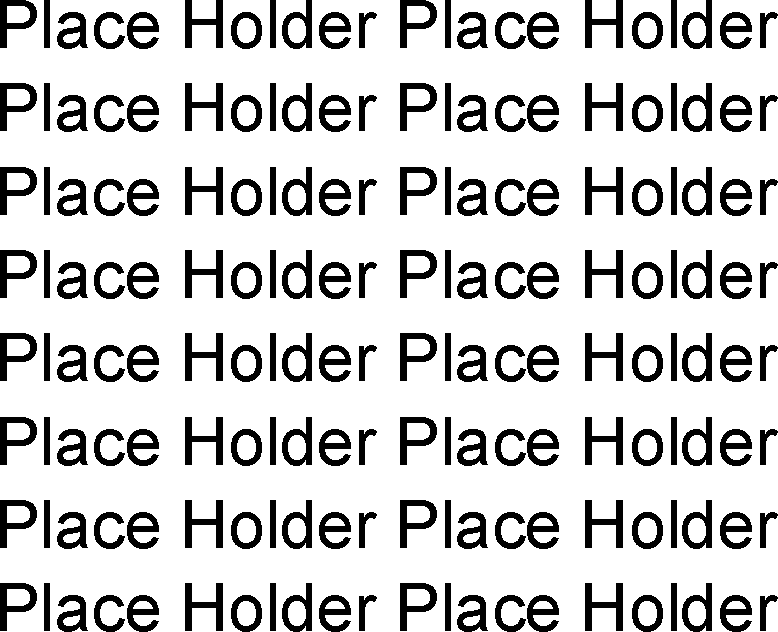
\includegraphics[scale=0.5]{imgs/place_holder.pdf}}
	\subfigure[Test subfigure 2]{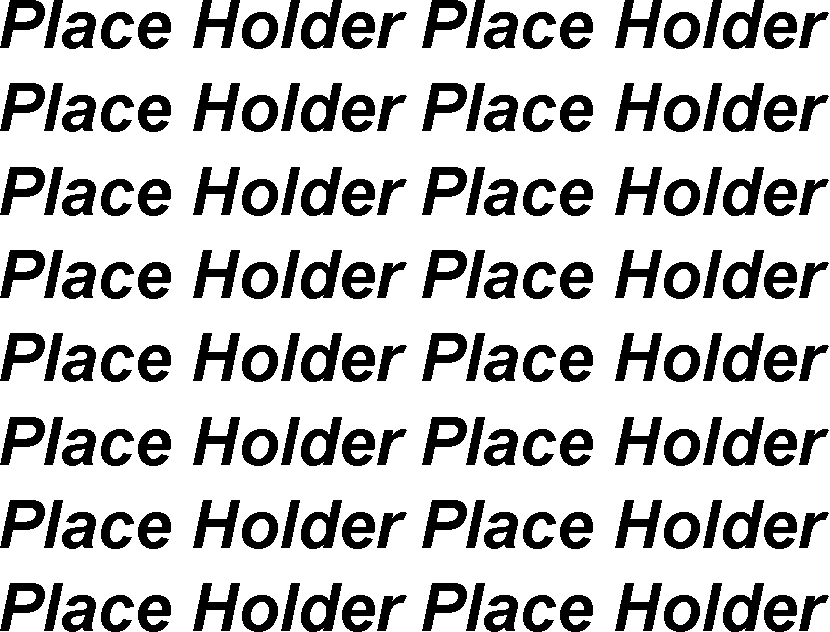
\includegraphics[scale=0.5]{imgs/place_holder_2.pdf}}
	}
    \renewcommand{\thefigure}{\thechapter.\arabic{figure}}
    \caption[]{Memory consumption in rendering phase.}
    \label{fig:pm_global} 
\end{figure}   

The following series of images groups rendered with our new approach is a frame sequence rendering a scene with moving point light source. The figure \ref{fig:pq_frame_1} frame is rendered with the point light located in the defualt position.  

\begin{figure}\label{fig:result_images}
\begin{center}
\setlength{\tabcolsep}{0mm}
\subfigure[]{%	Result Image
\begin{tabular}{c}
\includegraphics*[width=0.5\textwidth]{imgs/place_holder.pdf}\\
\includegraphics*[width=0.5\textwidth]{imgs/place_holder.pdf}\\
\includegraphics*[width=0.5\textwidth]{imgs/place_holder.pdf}
\end{tabular}
}%
\subfigure[]{%	Photons Visualization
\begin{tabular}{c}
\includegraphics*[width=0.5\textwidth]{imgs/place_holder.pdf}\\
\includegraphics*[width=0.5\textwidth]{imgs/place_holder.pdf}\\
\includegraphics*[width=0.5\textwidth]{imgs/place_holder.pdf}
\end{tabular}
}%

\caption{a caption}
\end{center}
\end{figure}

As shown in figure \ref{fig:result_images}, the quality of 	result images become better and finally stablized after a certain number of frames. It is not difficult to understand why we have such result according to our algorithm, as we trace fewer photons for each frame, the beginning few images apparently are less illuminated by the light source, in the following frames, we keep shooting and more photons into the scene and accumulating the photons to the photons queue. Therefore we can visualize more and more photons and the scene becomes brighter. The number of photons in the scene will become stable when the maximum frames, since there are same amount of photons traced as they are supposed to be compares to the standard approach. Eventually we will achieve same image quality as of the standard photon mapping. 


